\documentclass[border={10pt 5pt 5pt 5pt},tikz]{standalone}

\usepackage[T1]{fontenc}
\usepackage[sfdefault,scaled=.85]{FiraSans}
\usepackage{tikz}
\usepackage{pgfplots}
\usepackage{ifthen}
\usetikzlibrary{arrows.meta}
\usetikzlibrary{shapes.geometric}
\usetikzlibrary{mindmap,trees,shadows}

\usetikzlibrary{arrows.meta,angles,quotes}
\colorlet{linecol}{black!75}
\usepackage{forest}

\begin{document}

	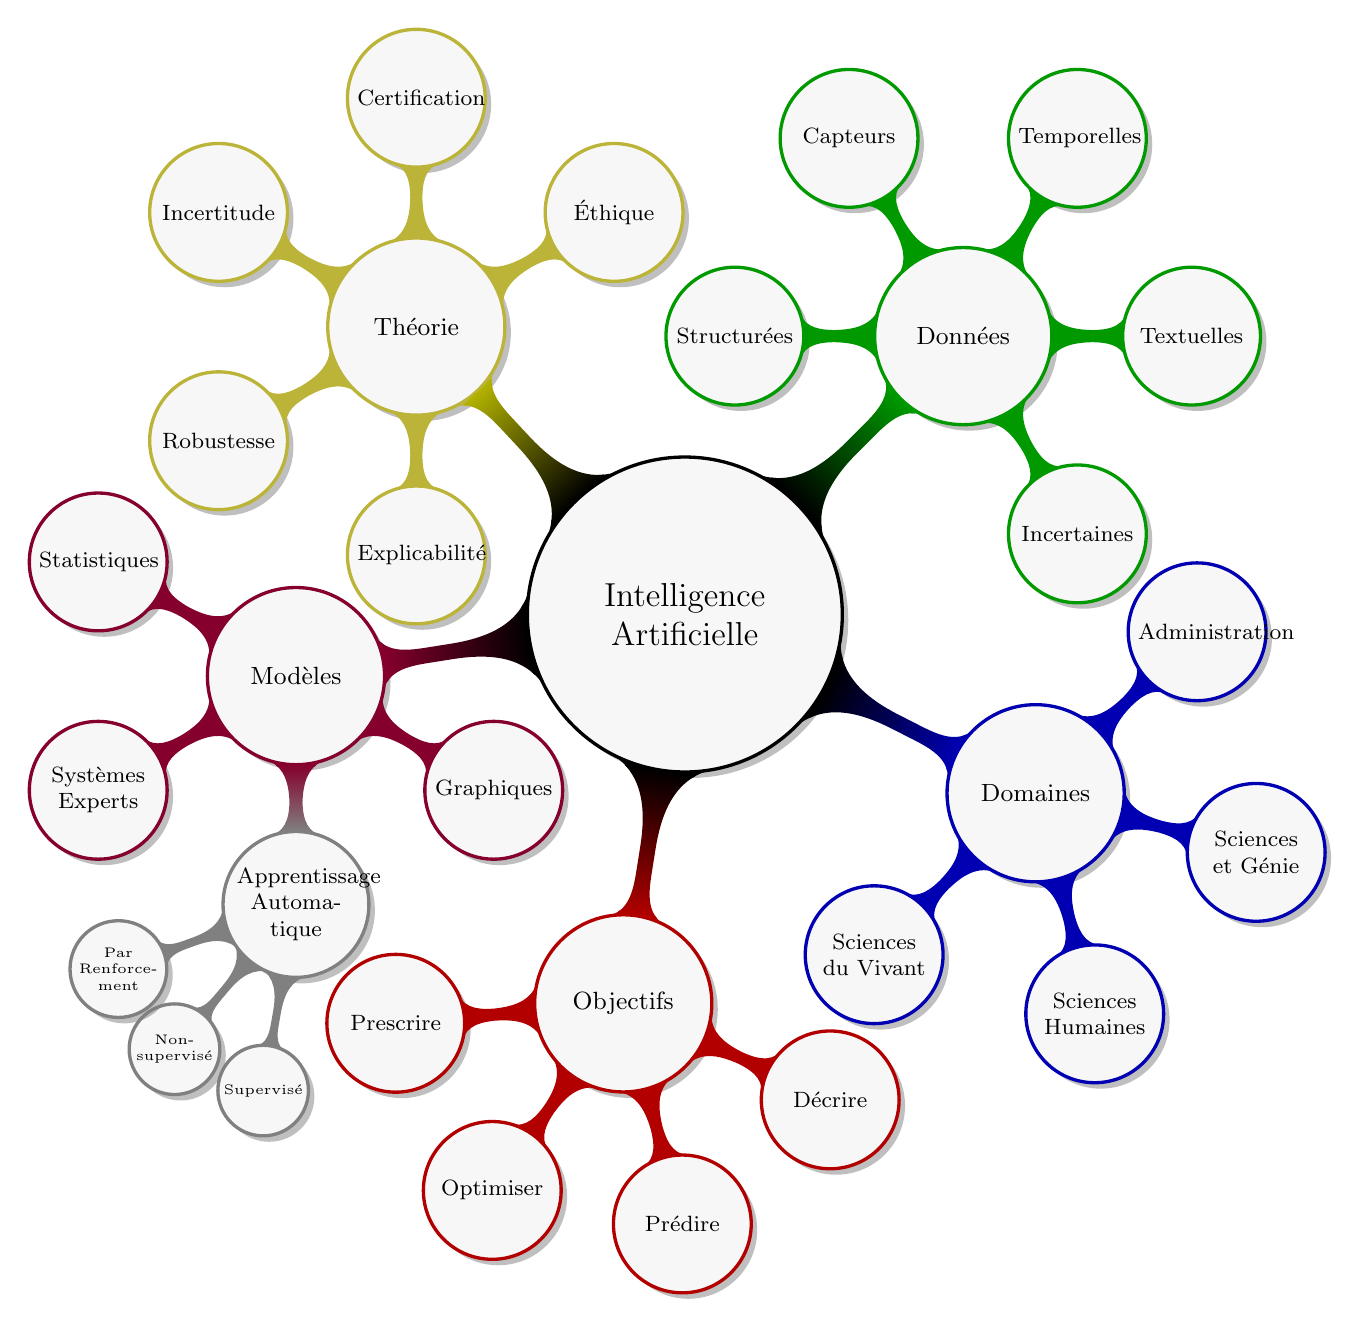
\begin{tikzpicture}
		\tikzset{concept/.append style={fill={black!3},drop shadow}}
		\path[mindmap,concept color=black,text=black]
		node[concept] {Intelligence Artificielle}
		[clockwise from=45]
		child[concept color=green!60!black] {
			node[concept] (data) {Données}
			[clockwise from=180]
			child { node[concept] (tab) {Structurées} }
			child { node[concept] (capt) {Capteurs} }
			child { node[concept] (temp) {Temporelles} }
			child { node[concept] (text) {Textuelles} }
			child { node[concept] (datunc) {Incertaines} }
		}
		child[concept color=blue!70!black, sibling angle=72] {
			node[concept] (domains) {Domaines}
			[clockwise from=45]
			child { node[concept,font=\footnotesize] (adm) {Administration} }
			child { node[concept] (sg) {Sciences et Génie} }
			child { node[concept] (sh) {Sciences Humaines} }
			child { node[concept] (sv) {Sciences du Vivant} }
		}
		child[concept color=red!70!black, sibling angle=72] {
			node[concept] (objs) {Objectifs}
			[clockwise from=-25]
			child { node[concept] (dec) {Décrire} }
			child[sibling angle=50] { node[concept] (pred) {Prédire} }
			child[sibling angle=50] { node[concept] (opt) {Optimiser} }
			child[sibling angle=50] { node[concept] (pres) {Prescrire} }
		}
		child[concept color=purple!70!black, sibling angle=72] { 
			node[concept] (models) {Modèles} 
			[clockwise from=-30]
			child { node[concept] (graph) {Graphiques} }
			child[concept color=gray] { 
				node[concept, font=\footnotesize] (ml) {Apprentissage Automatique} 
				[clockwise from=-100]
				child { node[concept] (sup) {Supervisé} }
				child { node[concept] (nsup) {Non-supervisé} }
				child { node[concept] (rl) {Par Renforcement} }
			}
			child { node[concept] (se) {Systèmes Experts} }
			child { node[concept] (stat) {Statistiques} }
		}
		child[concept color=yellow!70!black, sibling angle=68] { 
			node[concept] (theory) {Théorie} 
			[clockwise from=-90]
			child { node[concept] (expl) {Explicabilité} }
			child { node[concept] (rob) {Robustesse} }
			child { node[concept] (theunc) {Incertitude} }
			child { node[concept] (cert) {Certification} }
			child { node[concept] (eth) {Éthique} }
		};
\end{tikzpicture}

\end{document}
